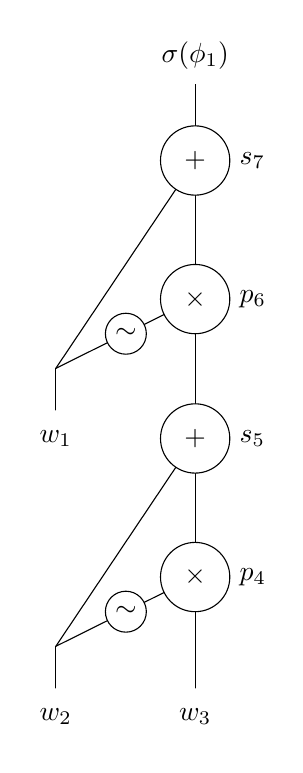
\begin{tikzpicture}
\definecolor{fillcolor}{RGB}{255,255,255}
\definecolor{highcolor}{RGB}{0,0,0}
\definecolor{lowcolor}{RGB}{0,0,0}
\definecolor{neutralcolor}{RGB}{0,0,0}
\definecolor{pathcolor}{RGB}{0,0,0}
\definecolor{background}{RGB}{225,225,225}
\draw (2.12,8.74) [thin,neutralcolor] -- (2.12,7.41);
\draw (2.12,7.41) [thin,neutralcolor] -- (0.35,4.77);
\draw (2.12,7.41) [thin,neutralcolor] -- (2.12,5.65);
\draw (2.12,5.65) [thin,neutralcolor] -- (0.35,4.77);
\draw [fill=neutralcolor,draw=neutralcolor] (1.24,5.21) circle [radius=0.09];
\draw (2.12,5.65) [thin,neutralcolor] -- (2.12,3.88);
\draw (2.12,3.88) [thin,neutralcolor] -- (0.35,1.24);
\draw (2.12,3.88) [thin,neutralcolor] -- (2.12,2.12);
\draw (2.12,2.12) [thin,neutralcolor] -- (0.35,1.24);
\draw [fill=neutralcolor,draw=neutralcolor] (1.24,1.68) circle [radius=0.09];
\draw (2.12,2.12) [thin,neutralcolor] -- (2.12,0.35);
\draw (0.35,4.77) [thin,neutralcolor] -- (0.35,3.88);
\draw (0.35,1.24) [thin,neutralcolor] -- (0.35,0.35);
\draw [thin,fill=fillcolor,draw=fillcolor] (2.12,8.74) circle [radius=0.35];
\node at (2.12,8.74) {$\sigma(\phi_1)$};
\draw [thin,fill=fillcolor,draw=neutralcolor] (2.12,7.41) circle [radius=0.44];
\node at (2.12,7.41) {$+$};
\draw [thin,fill=fillcolor,draw=neutralcolor] (2.12,5.65) circle [radius=0.44];
\node at (2.12,5.65) {$\times$};
\draw [thin,fill=fillcolor,draw=neutralcolor] (2.12,3.88) circle [radius=0.44];
\node at (2.12,3.88) {$+$};
\draw [thin,fill=fillcolor,draw=neutralcolor] (2.12,2.12) circle [radius=0.44];
\node at (2.12,2.12) {$\times$};
\draw [thin,fill=neutralcolor,draw=neutralcolor] (0.35,4.77) circle [radius=0.00];
\node at (0.35,4.77) {};
\draw [thin,fill=fillcolor,draw=fillcolor] (0.35,3.88) circle [radius=0.35];
\node at (0.35,3.88) {$w_1$};
\draw [thin,fill=neutralcolor,draw=neutralcolor] (0.35,1.24) circle [radius=0.00];
\node at (0.35,1.24) {};
\draw [thin,fill=fillcolor,draw=fillcolor] (0.35,0.35) circle [radius=0.35];
\node at (0.35,0.35) {$w_2$};
\draw [thin,fill=fillcolor,draw=fillcolor] (2.12,0.35) circle [radius=0.35];
\node at (2.12,0.35) {$w_3$};
\draw [thin,fill=fillcolor,draw=neutralcolor] (1.24,5.21) circle [radius=0.26];
\node at (1.24,5.21) {$\sim$};
\draw [thin,fill=fillcolor,draw=neutralcolor] (1.24,1.68) circle [radius=0.26];
\node at (1.24,1.68) {$\sim$};
\node [right] at (2.56,7.41) {$s_7$};
\node [right] at (2.56,5.65) {$p_6$};
\node [right] at (2.56,3.88) {$s_5$};
\node [right] at (2.56,2.12) {$p_4$};
\end{tikzpicture}%%
